\chapter{Tela de LCD (\textit{Liquid Crystal Display})}

    \begin{figure}[h]
    \caption{Tela LCD}
     
    \centering 
    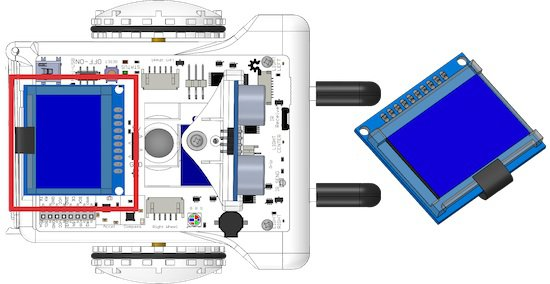
\includegraphics[width=9cm]{Figuras/Top_LCD1.jpeg}
    \label{figura:Top_LCD1.jpeg}
    \end{figure}

\section*{Introdução}
\paragraph{}
O \textit{Sparki} possui uma tela LCD onde é possível desenhar, escrever e visualizar dados de sensores em funcionamento. Ao olhar bem de perto, pode-se perceber que a tela é formada por pequenos pontos que podem ser programados para estarem em um de dois estados, ligado ou desligado. Nós chamamos esses pontos de \textit{pixels}. Eles também estão presentes em TVs, monitores de computador, celulares e eles são ligados ou desligados em uma disposição na qual seja possível formar uma imagem na tela. No caso do \textit{Sparki}, ele possui 128 \textit{pixels} na horizontal e 64 \textit{pixels} na vertical, e para identificar cada pixel deve ser fornecido a coordenada horizontal, vertical, e se ele deverá ficar aceso ou apagado. 

    \begin{figure}[h]
    \caption{Pixels}
     
    \centering 
    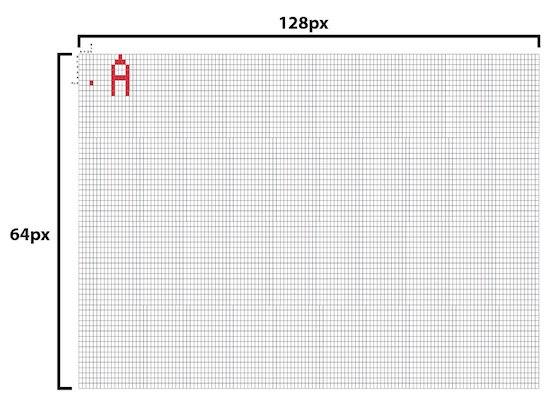
\includegraphics[width=9cm]{Figuras/LCD_Diagram1.jpg}
    \label{figura:LCD_Diagram1.jpg}
    \end{figure}
    
\section{Funções}

Para imprimir algo na tela LCD, você deve seguir 4 passos importantíssimos:
\begin{description}
\item[1.] Limpar o LCD --> \lstinline[columns=fixed]{sparki.clearLCD()}
\item[2.] Informar o que você quer que apareça no LCD -->
%não consegui arrumar a identação do código aqui. Talvez essa função não funcione bem dentro de tópicos.
\begin{lstlisting}[language=C]
sparki.drawLine(x,y,127,63);
sparki.drawRect(5,5, 30,10); 
sparki.drawRectFilled(15,17,30,10); 
sparki.drawCircle(20,45,12); 
sparki.drawCircleFilled(90,40,20); 
sparki.print("nao pula linha"); 
sparki.println("pula linha depois");
\end{lstlisting}

\item[3.] Atualizar a tela --> \lstinline[columns=fixed]{sparki.updateLCD()}
\item[4.] Criar um intervalo de tempo --> \lstinline[columns=fixed]{delay()}
\end{description}

\subsection{Passo 1: Limpar o LCD}

\paragraph{}
O primeiro passo para mostrar algo no LCD é limpar todas as informações que estão no armazenadas no \textit{Sparki} e, para isso, utilizamos a função \lstinline[columns=fixed]{sparki.clearLCD()}. Esta função não precisa de parâmetros, então não precisamos escrever nada dentro dos parênteses.

\begin{center}
    \textcolor{mydarkblue}{\textbf{Para não esquecer!}} 
    \\ ``Clear'' traduzido para o português significa ``limpar''.
\end{center}

\subsection{Passo 2: Informar ao LCD}

\paragraph{sparki.drawLine(xi, yi, xf, yf):} 
Esta função cria uma linha de acordo com o ponto de início e do fim do traço. Então \lstinline[columns=fixed]{xi} e \lstinline[columns=fixed]{yi} são as coordenadas do ponto de início do traço e \lstinline[columns=fixed]{xf} e \lstinline[columns=fixed]{yf} são as coordenadas do fim do traço.

\paragraph{sparki.drawRect(xi, yi, xf, yf):}
Esta função desenha um retângulo, sendo \lstinline[columns=fixed]{xi} e \lstinline[columns=fixed]{yi} coordenadas do canto superior esquerdo do retângulo e \lstinline[columns=fixed]{xf} e \lstinline[columns=fixed]{yf} coordenadas do canto inferior direito do retângulo.

\paragraph{sparki.drawRectFilled(xi, yi, xf, yf):}
Esta função é semelhante à \lstinline[columns=fixed]{sparki.drawRect(xi, yi, xf, yf)}, a única diferença é que ele desenha um retângulo preenchido.
 
\paragraph{sparki.drawCircle(xc, yc, raio):}
Esta função desenha um círculo de acordo com as coordenadas do centro e o raio. As coordenadas \lstinline[columns=fixed]{xc} e \lstinline[columns=fixed]{yc} indicam onde deve ficar o centro do círculo e o parâmetro \lstinline[columns=fixed]{raio} indica o tamanho do raio.
 
\paragraph{sparki.drawCircleFilled(xc, yc, raio):}
Esta função é semelhante à \lstinline[columns=fixed]{sparki.drawCircle(xc, yc, raio)}, a única diferença é que ele desenha um círculo preenchido.

\begin{center}
    \textcolor{mydarkblue}{\textbf{Para não esquecer!}} 
    \\ ``Draw'' traduzido para o português significa ``desenhar''.
    \\ ``Line'' traduzido para o português significa ``linha''.
    \\ ``Rect'' é uma abreviação de ``rectangle'', que traduzido para o português significa ``retângulo''.
    \\ ``Circle'' traduzido para o português significa ``círculo''.
    \\ ``Filled'' significa ``preenchido''.
\end{center}

\paragraph{sparki.print:} 
Com esta função, é possível imprimir caracteres e números na tela, basta escrever a mensagem a ser impressa dentro dos parênteses e das aspas. Essa função também é bastante utilizada para imprimir os valores recebidos dos sensores, mas, para essa utilidade, o parâmetro deverá ser uma variável* e o nome dela não será escrita entre aspas.
\par* No capítulo 5 iremos aprender mais sobre variáveis e seus usos, por isso, não vamos nos ater muito à funcionalidade do sparki.print(variavel), ok?
  
\paragraph{sparki.println:}
Assim como a função anterior, ela imprime uma mensagem na tela. A diferença é que essa função gera uma quebra de linha ao fim dessa mensagem.

\begin{center}
    \textcolor{mydarkblue}{\textbf{Para não esquecer!}} 
    \\ ``Print'' traduzido para o português significa ``imprimir''.
\end{center}

\subsection{Passo 3: Atualizar a tela do LCD}

\paragraph{}
A função \lstinline[columns=fixed]{sparki.updateLCD()} é importante para atualizar a tela, informando ao \textit{Sparki} que ele já pode mostrar no LCD as informações que foram passadas.

\begin{center}
    \textcolor{mydarkblue}{\textbf{Para não esquecer!}} 
    \\ ``Update'' traduzido para o português significa ``atualizar''.
\end{center}

\subsection{Passo 4: Criar um intervalo de tempo}
\paragraph{}
Para criar um intervalo de tempo, devemos utilizar a função \lstinline[columns=fixed]{delay()}. Ela não precisa de parâmetros.\\

\textit{Não entendi o porquê de precisarmos criar um intervalo de tempo. Não faz sentido!} \par
O intervalo de tempo é necessário para que a mensagem/imagem permaneça na tela por tempo suficiente para que possamos visualizá-la. Caso criemos um código para o LCD sem incluir esse passo, não conseguiremos visualizar na tela. Ficou confuso? Basta pensar que estamos limpando e atualizando o LCD com novas informações o tempo todo, então, os \textit{pixels} estão sendo ligados e desligados a cada vez que o \lstinline[columns=fixed]{void loop()} é lido. Por isso, queremos que as informações continuem sendo exibidas na tela (\lstinline[columns=fixed]{sparki.updateLCD()}) por mais tempo do que elas permanecem apagadas (\lstinline[columns=fixed]{sparki.clearLCD()}).

\begin{center}
    \textcolor{mydarkblue}{\textbf{Para não esquecer!}} 
    \\ ``Delay'' traduzido para o português significa ``demora'', ``atraso''.
\end{center}

\subsection{Exemplos}
\textsc{Exemplo 1)} Neste exemplo a tela LCD do \textit{Sparki} irá mostrar duas retas, uma partindo do canto superior esquerdo e indo até o canto inferior direito e outra partindo do canto superior direito e indo até o canto inferior esquerdo. E esse desenho será mostrado no LCD por 1 segundo antes do código ser repetido.

\begin{lstlisting}[language=C]
#include <Sparki.h>;

void setup()
{
}

void loop()
{
    sparki.clearLCD();
    sparki.drawLine(0,0,127,63);
    sparki.drawLine(0,63,127,0);        
    sparki.updateLCD();
    delay(1000);  
}
\end{lstlisting}

\textsc{Exemplo 2)} Agora vamos fazer um exemplo com o círculo preenchido. Neste caso, o raio do círculo é 10 e as coordenadas são as seguintes: x = 60, y = 30;

\begin{lstlisting}[language=C]
#include <Sparki.h>;

void setup()
{
}

void loop()
{
  sparki.clearLCD();
  sparki.drawCircleFilled(60,30,10);
  sparki.updateLCD();
  delay(1000);  
}
\end{lstlisting}

\textsc{Exemplo 3)} Neste exemplo, iremos visualizar um código que imprime um retângulo. 


\begin{lstlisting}[language=C]
#include <Sparki.h>;

void setup()
{
}

void loop()
{
  sparki.clearLCD();
  sparki.drawRect(10,15,20,25);
  sparki.updateLCD();
  delay(1000);  
}
\end{lstlisting}

Para começar, vamos analisar os parâmetros da função de desenhar um retângulo. Os dois primeiros parâmetros representam as coordenadas do ponto referente ao canto superior esquerdo, ou seja, xi = 10, yi = 15. Já os dois últimos, eles fazem referência ao ponto do canto inferior direito, ou seja, xf = 20, yf = 25. Note que a ordem dos parâmetros faz muita diferença quando se trata de funções.
\\~\\
\par \textsc{Exemplo 4)} Agora, veremos um exemplo de como imprimir caracteres na tela LCD por meio de aspas.
\begin{lstlisting}[language=C]
#include <Sparki.h>;

void setup()
{
}

void loop()
{
  sparki.clearLCD();
  sparki.println("Oi, eu sou o Sparki");
  sparki.print("Tudo bem");
  sparki.print("?");
  sparki.updateLCD();
  delay(1000);  
}
\end{lstlisting}

Perceba que em um dos comandos de imprimir caracteres tem um "ln", lembra o que isso significa? Isso significa que, após escrever os caracteres que estão entre as aspas, será pulada uma linha. Então ficaria mais ou menos assim:

\begin{table}[h]
 \centering
 {\renewcommand\arraystretch{1.5}
 \caption{Resultado no LCD}
 \begin{tabular}{ l }
  \cline{1-1}  
    \multicolumn{1}{|p{3.333cm}|}{Oi, eu sou o Sparki       Tudo bem?}
  \\  
  \hline
 \end{tabular} }
\end{table}

\section{Exercícios}

\question{Crie um código que desenhe no centro da tela LCD do Sparki um círculo de raio 20 e, no centro dele, um círculo preenchido de raio 10. Dica: lembre-se das proporções dessa tela LCD.}
    \begin{center}
    \line(1,0){450}
    \vspace{0.2cm}   
    \line(1,0){450}
    \vspace{0.2cm}   
    \line(1,0){450}
    \vspace{0.2cm}   
    \line(1,0){450}
    \vspace{0.2cm}   
    \line(1,0){450}
    \vspace{0.2cm}   
    \line(1,0){450}
    \vspace{0.2cm}   
    \line(1,0){450}
    \vspace{0.2cm}   
    \line(1,0){450}
    \vspace{0.2cm}   
    \line(1,0){450}
    \vspace{0.5cm}   
    \end{center}

\question{Marque qual das alternativas é equivalente à mensagem que será exibida na tela do \textit{Sparki} após o seguinte código ser lido:}

\begin{lstlisting}[language=C]
#include <Sparki.h>;

void setup()
{
}

void loop()
{
  sparki.clearLCD();
  sparki.print("Ola ");
  sparki.println("humanos!");
  sparki.print("Eu me");
  sparki.print("chamo ");
  sparki.println("Sparki");
  sparki.updateLCD();
  delay(1000);  
}
\end{lstlisting}

\begin{enumerate}
        \item Ola humanos!Eu me chamo Sparki
        \item Ola \\
        humanos! Eu me chamo \\
        Sparki
        \item Ola humanos! \\
        Eu me chamo Sparki
        \item Ola humanos! \\
        Eu mechamo Sparki
    \end{enumerate}

\question{Responda qual seria a altura e o comprimento do retângulo impresso na tela LCD (em pixels), com base no seguinte código:}

\begin{lstlisting}[language=C]
#include <Sparki.h>;
void setup()
{
}
void loop()
{
  sparki.clearLCD();
  sparki.drawRect(10,15,35,25);
  sparki.updateLCD();
  delay(1000);  
}
\end{lstlisting}

a) Altura do retângulo:
\begin{center}
    \line(1,0){450}
    \vspace{0.3cm}   
\end{center}
b) Comprimento do retângulo:
\begin{center}
    \line(1,0){450}
    \vspace{0.5cm}   
\end{center}

\challenge{Crie um código que imprima um rosto na tela LCD do Sparki, de forma que os olhos sejam círculos preenchidos e a boca seja um retângulo. As proporções ficam a seu critério.}
\begin{center}
    \line(1,0){450}
    \vspace{0.2cm}   
    \line(1,0){450}
    \vspace{0.2cm}   
    \line(1,0){450}
    \vspace{0.2cm}   
    \line(1,0){450}
    \vspace{0.2cm}   
    \line(1,0){450}
    \vspace{0.2cm}   
    \line(1,0){450}
    \vspace{0.2cm}   
    \line(1,0){450}
    \vspace{0.2cm}   
    \line(1,0){450}
    \vspace{0.2cm}   
    \line(1,0){450}
    \vspace{0.5cm}   
\end{center}
